In initial tests, basic components were mounted to the drone using simple mounting tape. In later tests, a more robust solution was required. Because of the specific component set, Joshua created a lightweight mounting plate to accommodate both the components and an overhead canopy. A canopy designed for the Tarot 680 was conveniently available directly on Thingiverse \cite{canopy_thingiverse}, and it provides physical protection of the onboard electronics from moisture, dust, and other debris. A mounting plate for the components (shown in Figure \ref{fig:component_mounting_plate}) was designed to fit the top plate of the drone. It mounts using screws in the unused holes in the top of the drone's plate. Larger screw holes allow the plate to sit flush against the drone's top plate even with the existing screws which stick up slightly. These screws also help to keep the mounting plate in place laterally. Larger central holes allow wires to pass through the plate from the center to the electronics. Standoffs provide a well-organized and stable mounting point for the flight controller and companion boards. The vertical plates on the side provide a mounting place for the RC receiver and BEC. The hinge in the back connects to the corresponding hinge on the canopy, and the slit in the front allows a Velcro strap to hold the canopy closed. The hole in the canopy allows the GPS antenna to be mounted externally. An additional hole was made to accommodate the antenna for the telemetry radio. A specific mounting plate was created for each drone because the mounting holes for the companion boards are different, but the mounting plates are otherwise the same. The mounting plates and canopies were printed and installed on the drones iteratively, with slight changes each time. This was designed in OpenSCAD and all .stl and .scad files are available on Thingiverse \cite{mounting_plate_thingiverse}.

\begin{figure}
    \centering
    \includegraphics[width=0.7\textwidth]{images/mounting_plate_iterations.JPG}
    \caption{Iterations of the mounting plate design. The mounting plate was changed over time to be more lightweight and allow flexible placement of data and power cables.}
    \label{fig:mounting_plate_iterations}
\end{figure}

\begin{figure}
    \begin{subfigure}[b]{0.48\textwidth}
        \centering
        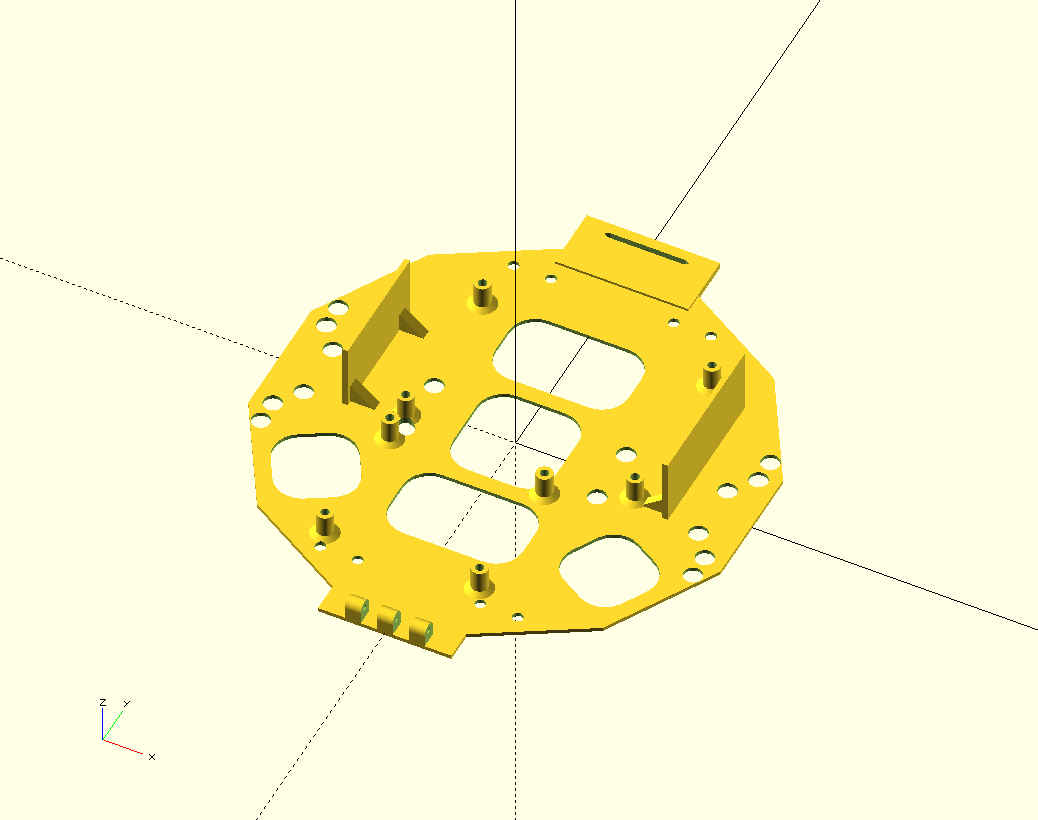
\includegraphics[width=\textwidth]{images/component_mounting_plate.png}
        \caption{Component mounting plate.}
        \label{fig:component_mounting_plate}
    \end{subfigure}
    \begin{subfigure}[b]{0.48\textwidth}
        \centering
        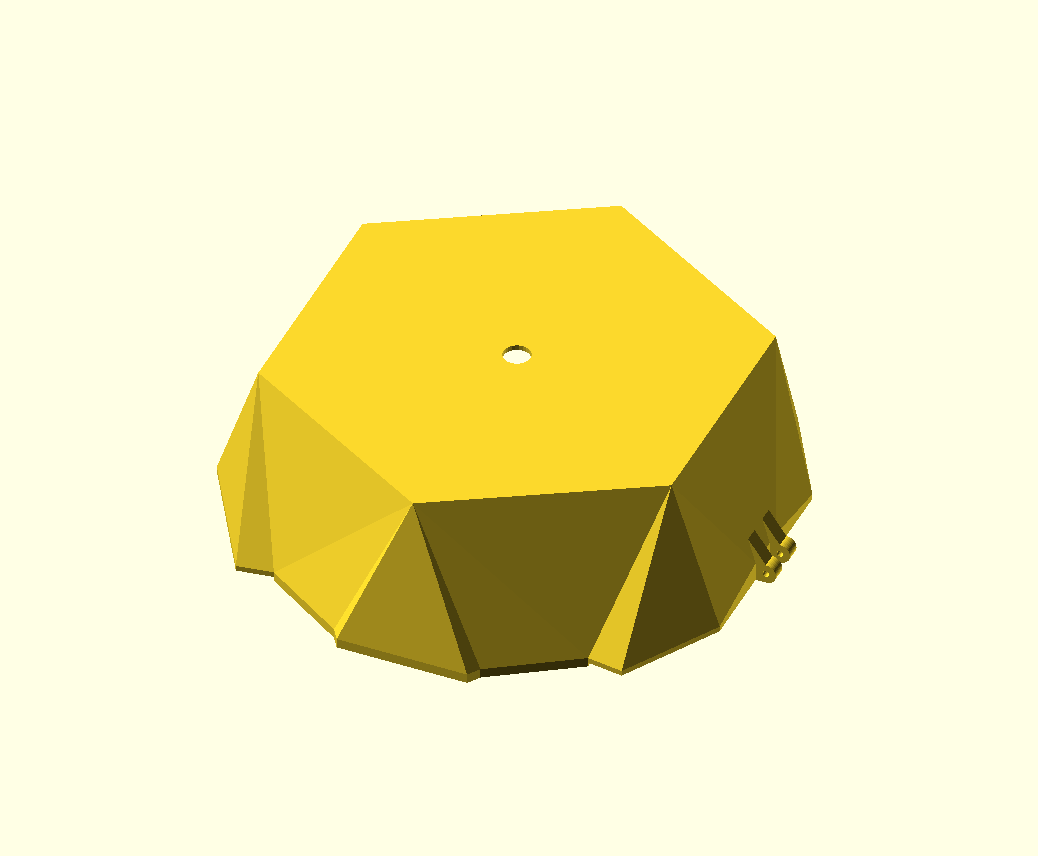
\includegraphics[width=\textwidth]{images/canopy.png}
        \caption{The canopy top for the electronics.}
        \label{fig:canopy}
    \end{subfigure}
    \caption{The final mounting plate and canopy cover.}
    \label{fig:mounting}
\end{figure}